\documentclass{article}

% NeurIPS 2025 formatting
%\usepackage{neurips_2025}
\usepackage[preprint]{neurips_2025} % Using preprint for draft
\usepackage{natbib}
\bibliographystyle{plainnat} % Moved bibliographystyle here for clarity

% Additional packages
\usepackage[utf8]{inputenc} % allow utf-8 input
\usepackage[T1]{fontenc}    % use 8-bit T1 fonts
\usepackage{hyperref}       % hyperlinks
\hypersetup{
    colorlinks=false,   % Don't color the links
    pdfborder={0 0 0},  % No border around links (set to 0)
    hidelinks           % Hide all visual cues of links
}
\usepackage{url}            % simple URL typesetting
\usepackage{booktabs}       % professional-quality tables
\usepackage{amsfonts}       % blackboard math symbols
\usepackage{nicefrac}       % compact symbols for 1/2, etc.
\usepackage{microtype}      % microtypography
\usepackage[usenames,dvipsnames]{xcolor}      % colors
\usepackage{amsmath,amssymb,amsthm}
\usepackage{enumitem}
\usepackage{geometry}       % For layout adjustments if needed
\usepackage{graphicx}
\usepackage{tikz} % Retained if complex figures are drawn with TikZ
\usetikzlibrary{arrows.meta,positioning,fit,backgrounds,calc} % Retained
\graphicspath{{./figures/}{./paper/images/}} % Adjusted graphics path to include 'figures/'

%%%% Macros
\newcommand{\Loss}{\mathcal{L}}
\newcommand{\R}{\mathbb{R}}
\newcommand{\E}{\mathbb{E}}
\newcommand{\He}{\mathrm{He}} % Retained from original

% Comments:
\newcommand{\giulia}[1]{{\color{ForestGreen}\textbf{Giulia:} #1}}
\newcommand{\mf}[1]{\todo[color=orange!30,size=\tiny]{MF: #1}}
\newcommand{\keivan}[1]{\todo[color=blue!30,size=\tiny]{K1: #1}}
\newcommand{\ff}[1]{\todo[color=blue!30,size=\tiny]{FF: #1}}
\newcommand{\AJ}[1]{\todo[color=green!30,size=\tiny]{AJ: #1}}
\usepackage[textsize=tiny]{todonotes} % Retained

%%%% Theorem environments (strategic use)
\newtheorem{theorem}{Theorem}[section]
\newtheorem{proposition}{Proposition}[section]
\newtheorem{lemma}{Lemma}[section]
\newtheorem{corollary}{Corollary}[section]
\newtheorem{definition}{Definition}[section]
\newtheorem{remark}{Remark}[section]
\newtheorem{observation}{Observation}[section]
\newtheorem{example}{Example}[section]


\title{Barriers for Learning in an Evolving World: \\a Mathematical Understanding of Loss of Plasticity}

\author{%
  Amir Joudaki$^{1}$ \And
  Giulia Lanzillotta$^{1}$ \And
  Mohammad Samragh Razlighi$^{2}$ \And
  Iman Mirzadeh$^{2}$ \And
  Keivan Alizadeh$^{2}$ \And
  Thomas Hofmann$^{1}$ \And
  Mehrdad Farajtabar$^{2}$ \And
  Fartash Faghri$^{2}$ \\
  $^{1}$ETH Zürich \\
  $^{2}$Apple \\
  \texttt{amir.joudaki@inf.ethz.ch},
  \texttt{\{fartash, farajtabar\}@apple.com}
}

\begin{document}
\maketitle

\begin{abstract}
    Standard deep learning models excel when trained on stationary datasets but often falter in non-stationary environments where continuous adaptation is crucial. This paradigm struggle is significantly due to the degradation of future learning capacity, a phenomenon termed loss of plasticity (LoP). This work undertakes a first-principles investigation into the mechanisms underlying LoP in gradient-based models. We propose a formal definition of LoP grounded in dynamical systems theory, identifying stable manifolds in the parameter space that act as traps for gradient trajectories. Our analysis details two specific mechanisms leading to such traps: frozen units arising from activation saturation and cloned-unit manifolds resulting from representational redundancy. Furthermore, we explore conditions under which architectural choices or targeted perturbations might prevent or mitigate this plasticity collapse.
    A core finding of our theoretical framework is the revelation of a fundamental tension: properties widely considered beneficial for generalization in conventional, static learning regimes, often characterized by distinct training and deployment phases, such as the emergence of low-rank representations or inherent simplicity biases, appear to directly contribute to LoP in continual learning scenarios.
    By mathematically characterizing these barriers, this work pinpoints critical representational properties that hinder continuous learning, providing a clear direction for developing truly adaptive artificial intelligence.
    Our theoretical analysis is supported by numerical simulations and empirical observations on various neural network architectures.
\end{abstract}

\section{Introduction}

The extraordinary success of back-propagation in training deep neural networks often relies on two implicit, yet critical, assumptions. First, \emph{stationarity}: the data distribution encountered during training is assumed to be identical, or very similar, to the distribution faced during deployment, rendering post-training adaptation minimal or absent. Second, \emph{single random initialization}: diversity and exploration potential are primarily introduced through a single random initialization of network parameters, a resource that is progressively consumed by optimization and not replenished. These assumptions falter when an artificial agent must operate and learn continuously within an environment characterized by changing dynamics or evolving task distributions. This scenario, often termed continual or lifelong learning, presents a significant challenge known as the stability-plasticity dilemma \citep{abraham2005memory, chaudhry2018riemannian}: the system must be stable enough to retain previously acquired knowledge, yet plastic enough to integrate new information effectively.

Empirically, standard deep networks subjected to long sequences of tasks or slowly drifting data streams often exhibit a decline in their learning capability \citep{dohare2024loss, berariu2021plasticity, dohare2021continual, nikishin2022primacy, lyle2023understanding}. This phenomenon, termed loss of plasticity (LoP), is distinct from catastrophic forgetting \citep{mccloskey1989catastrophic, ratcliff1990connectionist, french1999catastrophic}, where new learning overwrites old knowledge. LoP specifically refers to the diminished ability to learn new information effectively over time. Common symptoms include exploding weight magnitudes \citep{nikishin2022primacy}, activation saturation, the emergence of ``dead'' ReLU units (whose upstream parameters cease to update) \citep{nair2010rectified, sokar2023dormant, dohare2021continual, lyle2022understanding}, a collapse in the effective rank of hidden layer representations indicating reduced feature diversity \citep{papyan2020prevalence, huh2022lowrank, kumar2020implicit, gulcehre2022empirical}, and redundancy or diminishing contributions from network components like attention heads or filters \citep{lyle2023understanding}. Many of these issues have been highlighted in recent studies focusing on LoP \citep{dohare2023maintaining, kumar2024regenerative, ash2020warmstarting}.

\citet{dohare2024loss} argue compellingly that such failures are intrinsically linked to the back-propagation algorithm itself. They posit that gradient descent, optimized for transient, single-task learning, relies heavily on the initial random state for exploration, a resource that is consumed and not replenished during prolonged training. Their work demonstrates that standard deep learning methods can lose plasticity until they perform comparably to linear networks, and suggests that maintaining plasticity requires mechanisms beyond pure gradient descent, such as continually injecting diversity via methods like their proposed continual backpropagation.

\paragraph{Goal of this paper.}
Motivated by these observations, our paper revisits the dynamics of gradient descent and back-propagation through the lens of dynamical systems theory. We seek to answer the fundamental question:
\begin{quote}
\emph{What structural features inherent in gradient flow dynamics inevitably lead to LoP, and how might we design algorithms or architectures capable of perpetual adaptation?}
\end{quote}
The central proposition advanced in this work is that the tendency of gradient-based optimization to favor low-rank or ``simple'' representations lies at the heart of plasticity loss. While properties like low effective rank and simplicity bias are often associated with improved generalization in the standard two-phase learning paradigm \citep{huh2022lowrank, papyan2020prevalence, zhang2017understanding}, we argue that these very properties become detrimental in continual learning settings. By reducing the effective dimensionality of the network's feature space, they limit its capacity to adapt to novel information, thus contributing to the LoP observed by \citet{dohare2024loss} and others.

\section{Preliminaries}
\label{sec:preliminaries}

Let $\theta\in\Theta\subseteq\R^p$ represent the parameters of a neural network. We consider training on a stream of data $\{(x_i,y_i)\}_{i=1}^N$ using gradient descent or its stochastic variants. The objective is typically to minimize a loss function $\sum_{i=1}^N \Loss(\hat{y}_\theta(x_i),y_i),$ which we denote as $\Loss(\theta)$. The learning dynamics can be idealized by the continuous-time gradient flow:
\begin{equation}
    \frac{d\theta(t)}{dt} \;=\; -\nabla_\theta\Loss\bigl(\theta(t)\bigr).
    \label{eq:grad_flow}
\end{equation}
This perspective allows us to analyze the trajectory of parameters $\theta(t)$ in the parameter space $\Theta$.

We introduce the concept of a LoP manifold to formalize the idea of gradient trajectories becoming trapped in lower-dimensional subspaces, thereby restricting future learning capacity.

\begin{definition}[LoP manifold]
\label{def:lop_manifold_main}
A manifold $\mathcal{M}\subset\Theta$ induces Loss of Plasticity (LoP) if the gradient of the loss function is tangent to the manifold at every point on the manifold. That is, $\nabla_\theta\Loss(\theta)\in T_\theta\mathcal{M}$ for all $\theta\in\mathcal{M}$, where $T_\theta\mathcal{M}$ denotes the tangent space of $\mathcal{M}$ at $\theta$. This ensures that once the gradient flow enters $\mathcal{M}$, it remains within $\mathcal{M}$.
\end{definition}

\begin{remark}
If the conditions in Definition~\ref{def:lop_manifold_main} hold irrespective of the specific data distribution generating the loss $\Loss$, we refer to it as structural LoP. If the conditions hold for a particular data distribution, it is a data-dependent LoP. This paper primarily focuses on structural LoP.
\end{remark}

\paragraph{Feed-forward Neural Networks.}
A feed-forward neural network computes outputs through a sequence of layers. For a node $v$, its post-activation $h(v)$ is $f_v (z(v))$, where $z(v) = \sum_{u: (u,v)\in E}w_{u,v}\,h(u)$ is its pre-activation, $f_v$ is its activation function, and $w_{u,v}$ are weights. Input nodes $V_{\text{in}}$ receive external inputs $x_v$.
The back-propagation algorithm computes gradients $\partial\Loss/\partial w(u,v)$ using error signals $\delta(v)$. For an output node $v \in V_{\text{out}}$, $\delta(v)=\partial\Loss/\partial h(v)$. For other nodes, $\delta(v)=\sum_{k\in\mathrm{out}(v)}\delta(k)\,w(v,k)\,f'_k(z(k))$. The gradient is $\partial\Loss/\partial w(u,v)=\delta(v)\,f'_v(z(v))\,h(u)$.
(A more formal definition can be found in Appendix~\ref{app:model_definition}.)

\section{Emergence of LoP Features}
\label{sec:emergence_lop}

The path towards understanding LoP begins with how neural network representations evolve during training. We argue that a fundamental tension between mechanisms that reduce representational complexity (e.g., for generalization in static settings) and those that maintain diversity (essential for adaptation) is at the core of LoP.

\paragraph{Linear Layers and Rank Reduction.}
Linear transformations, such as those in fully connected or convolutional layers (without their activations), generally tend to reduce or maintain the effective rank of representations. The \emph{effective rank} of a set of features can be thought of as a measure of their dimensionality or diversity, often quantified using the singular value distribution of the feature matrix (e.g., participation ratio \citep{roy2007effective}).
\begin{itemize}
    \item \textbf{Matrix Products:} The hard rank of a product of matrices ($AB$) cannot exceed the minimum of their individual ranks. Iterated matrix products, as in deep linear networks, can lead to a rapid collapse in rank.
    \item \textbf{Conditioning:} Products of matrices can also worsen the condition number, making the effective rank decrease even if the hard rank is maintained.
    \item \textbf{Random Matrices:} A chain of random matrices often converges to a rank-1 matrix \citep{o2006random}, illustrating an inherent tendency towards rank collapse in linear systems.
\end{itemize}

\paragraph{Non-linear Activations and Rank Improvement.}
In contrast, non-linear activation functions are crucial for improving representational capacity.
\begin{observation}
Non-linear activations can:
\begin{enumerate}
    \item Improve the \textbf{hard rank} of feature sets. If features are element-wise processed by a sufficiently non-linear function, their linear dependencies can be broken. (A formal proposition regarding this is often based on the properties of Vandermonde-like matrices formed by non-linear transformations; details in Appendix~\ref{app:theory_details}).
    \item Improve the \textbf{effective rank} and de-correlate features or samples. This improvement is often a function of how "effectively non-linear" the activation function is in the regime it operates. (Formal analysis, e.g., Proposition~\ref{prop:rank_recovery_nonlinear} later, supports this for Gaussian pre-activations).
\end{enumerate}
\end{observation}

\paragraph{Modulating Effective Non-linearity.}
The pre-activation statistics (mean, scale, range) significantly influence an activation's effective non-linearity.
Consider $f(x) = \tanh(ax)$. If $a$ is small, $\tanh(ax) \approx ax$, behaving linearly. If $a$ is large, $\tanh(ax) \approx \mathrm{sign}(x)$, a highly non-linear function. Similarly, for $f(x) = \mathrm{ReLU}(ax+b)$: if $b$ is large and positive, $f(x) \approx ax+b$ (affine) for many inputs. If $b$ is large and negative, $f(x) \approx 0$ (dead).
The ability of an activation to increase rank depends on it operating in a genuinely non-linear regime.

\begin{figure}[ht!]
    \centering
    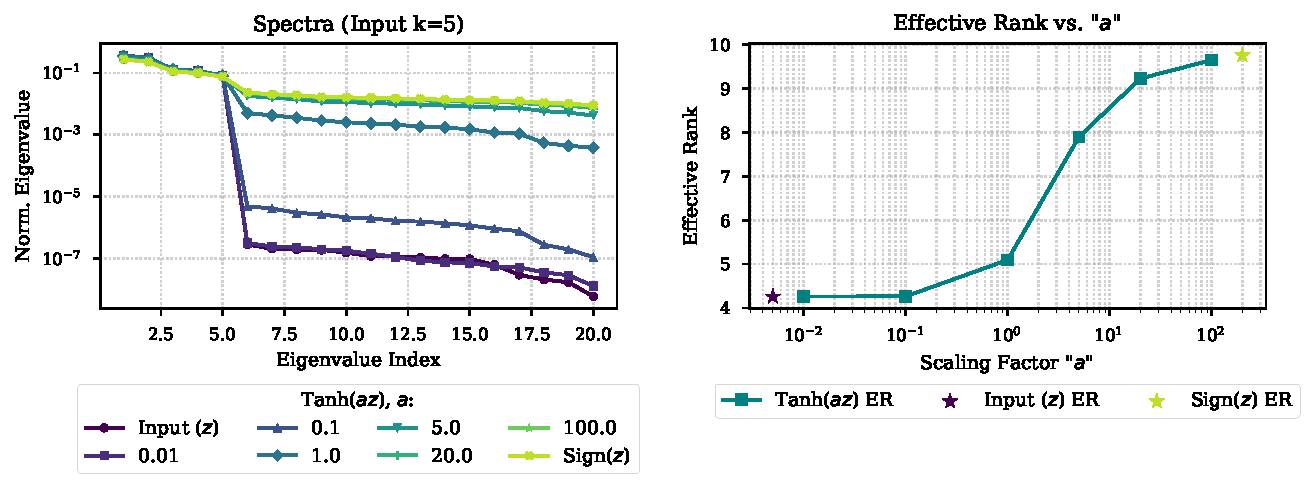
\includegraphics[width=0.7\linewidth]{figures/theory_tanh_az_rank.pdf}
    \caption{Effect of input scaling on post-activation effective rank for $h = \tanh(az)$, with rank-deficient $z$. Small $a$ leads to linear behavior and minimal rank increase. Appropriate $a$ enhances non-linearity and rank recovery. (Details in Appendix~\ref{app:additional_empirical_rank_figures})}
    \label{fig:theory_tanh_az_rank_main}
\end{figure}

\paragraph{Maximal Rank Increase and Saturated Units.}
What if we try to maximize an activation's rank-increasing capability? If an activation $f$ (or its derivative $f'$) is bounded, and we parametrize it to achieve an "infinitely non-linear" coefficient (e.g., $a \to \infty$ in $\tanh(ax)$), its derivative $f'$ often tends to zero almost everywhere under typical (e.g., Gaussian) pre-activation distributions.
\begin{itemize}
    \item For $\tanh(ax)$ or $\mathrm{sigmoid}(ax)$, as $a \to \infty$, the function saturates, and its derivative is zero except near $x=0$. These are \emph{frozen units}.
    \item For $\mathrm{ReLU}(ax+b)$, if $a$ is small and $b$ is a large negative value such that $ax+b$ is almost always negative, the unit is almost always "dead", with $f'(ax+b)=0$.
\end{itemize}

This paints a picture of a fundamental trade-off:
\begin{itemize}
    \item To increase rank and feature diversity, highly non-linear activations are needed. However, maximizing this non-linearity for a given activation often leads to saturation or freezing, where gradients vanish.
    \item To decrease rank (e.g., to compress information or due to simplicity bias), networks might reduce effective non-linearity (operating in near-linear regimes) or create duplicate/highly correlated features. Both hard and effective rank recovery mechanisms require non-duplicate features to function optimally.
\end{itemize}

\paragraph{The Role of Normalization.}
Normalization layers (e.g., BatchNorm, LayerNorm) standardize pre-activation statistics.
Without learnable affine parameters, they ensure consistent mean and scale. With learnable affine parameters ($ax+b$ after normalization, typically initialized to $a=1, b=0$), experiments suggest these parameters often act to constrain shifts in pre-activation statistics rather than driving them into extreme regimes.
Consequently, normalization generally helps maintain feature rank during training by:
\begin{enumerate}
    \item Preventing activations from operating too frequently in saturated (low-gradient) or overly linear (low rank-recovery) regimes.
    \item Keeping activations in a "healthy" non-linear range, thus preventing excessive rank recovery (which might risk saturation) or insufficient rank recovery (risking loss of diversity).
\end{enumerate}

\paragraph{Empirical Evidence of LoP Symptoms.}
During prolonged training, particularly in continual learning settings, networks often exhibit symptoms indicative of these underlying dynamics. Figure~\ref{fig:lop_emergence_continual_placeholder} illustrates the typical degradation: effective rank of representations plummets, while the fraction of duplicate features and frozen/dead units increases over tasks. Normalization layers tend to mitigate these effects.

\begin{figure}[ht!]
    \centering
    \textbf{[Placeholder for Figure: `fig:lop_emergence_continual`]}
    \caption{Conceptual illustration: During continual learning on Tiny ImageNet (classes partitioned into sequential tasks, 500 epochs/task), metrics like effective rank often decrease, while frozen/duplicate units increase over time. Normalization layers (e.g., BatchNorm) typically alleviate these trends. (Detailed experimental setup and more results in Appendix~\ref{app:empirical_details})}
    \label{fig:lop_emergence_continual_placeholder}
\end{figure}

\begin{figure}[ht!]
    \centering
    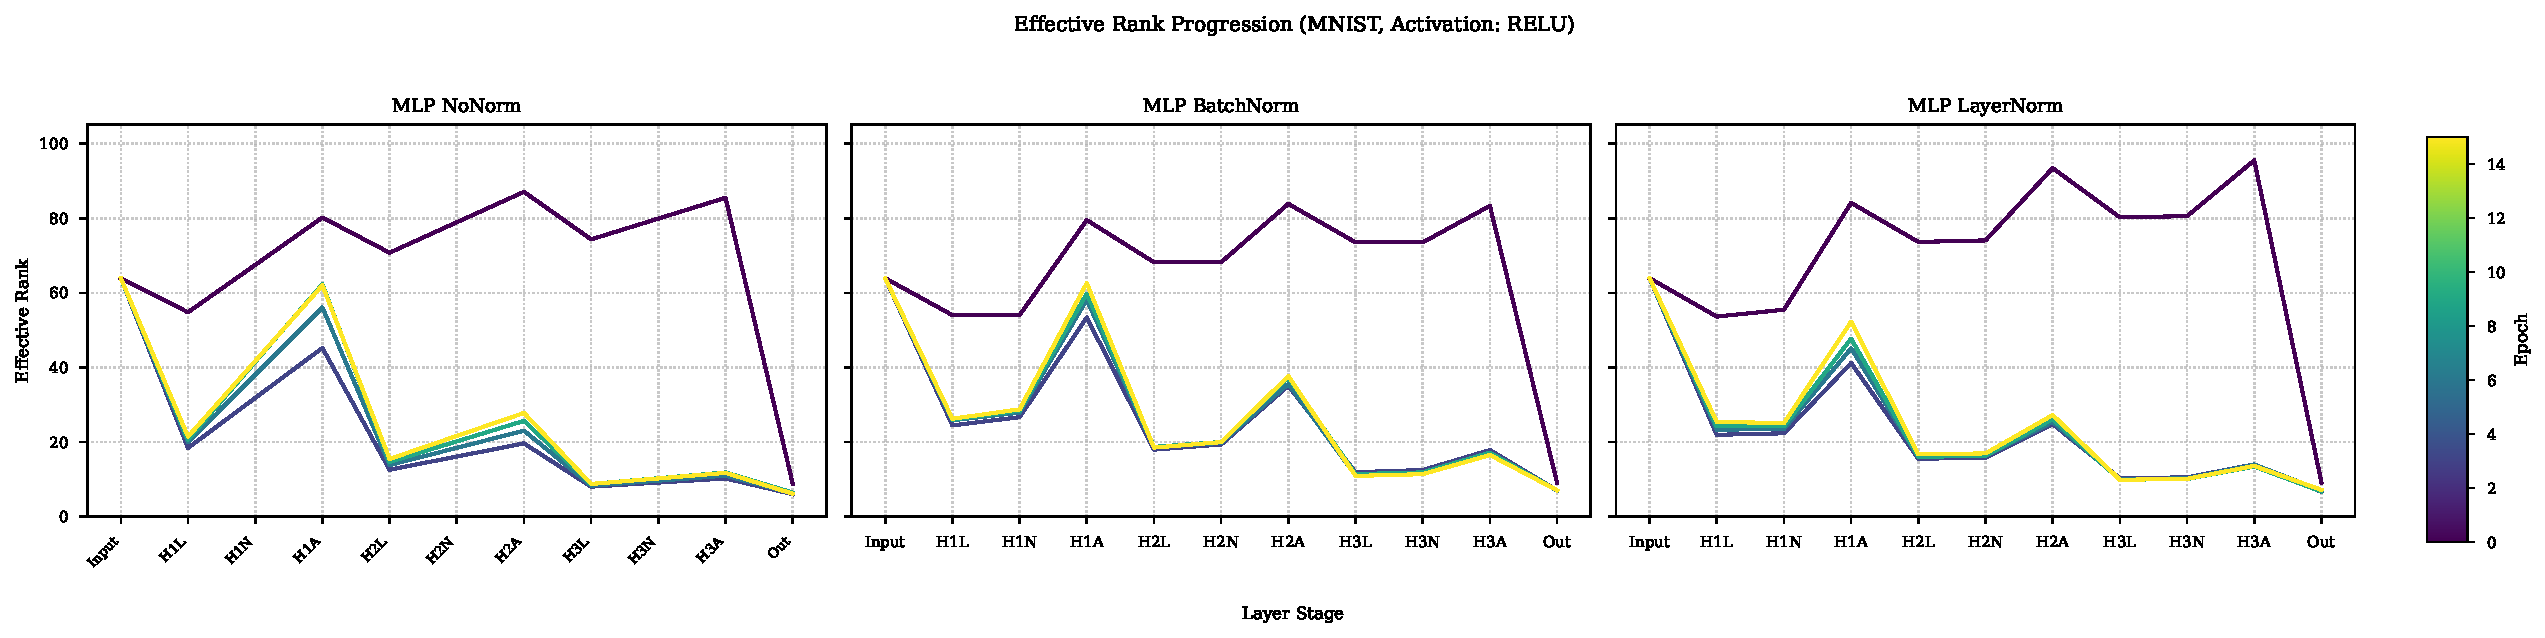
\includegraphics[width=\textwidth]{figures/empirical_rank_progression_relu_mnist.pdf}
    \caption{Empirical effective rank progression in an MLP trained on MNIST with ReLU activations, comparing no normalization, Batch Normalization, and Layer Normalization. Normalization helps maintain higher effective rank across layers and epochs. (Details in Appendix~\ref{app:additional_empirical_rank_figures})}
    \label{fig:empirical_rank_progression_main}
\end{figure}

(Further empirical evidence across various models and training regimes is detailed in Appendix~\ref{app:empirical_details}.)

\paragraph{Key Inferences from Emergence Dynamics.}
Our inquiry so far points to two primary types of problematic features emerging from training dynamics:
\begin{itemize}
    \item \textbf{Duplicate or highly correlated features:} Arising from attempts to lower representational rank or complexity.
    \item \textbf{Frozen or dead features:} Arising from attempts to maximize rank increase (leading to saturation) or to flatten the loss landscape around the current parameters.
\end{itemize}
A critical question remains: do these features lead to persistent LoP, as defined by our framework?

\section{Existence and Stability of LoP Manifolds}
\label{sec:existence_lop_manifold}

The emergent features discussed above can trap network parameters in LoP manifolds. We now formalize this.

\begin{proposition}[Formation of LoP Manifolds]
\label{prop:lop_manifold_formation}
Parameter subspaces characterized by either (1) frozen units or (2) cloned/duplicate units can form LoP manifolds as per Definition~\ref{def:lop_manifold_main}.
\begin{enumerate}
    \item \textbf{Frozen Units:} If a set of neurons becomes permanently saturated (e.g., $f'(z)=0$ for all relevant inputs), their incoming weights $\Theta_{\text{up}}$ cease to receive gradient updates. The parameters $\theta$ are then confined to a manifold where these $\Theta_{\text{up}}$ components are fixed. (Based on \citet{draft_placeholder_saturated_prop})
    \item \textbf{Cloned Units:} If a network possesses sets of units (clones) that are initialized and subsequently updated symmetrically such that their activations and outgoing weight contributions are identical, the network effectively behaves like a smaller network. The parameters are confined to an affine subspace where this symmetry is preserved. (Based on \citet{draft_placeholder_cloned_prop}; formal conditions on weight sums in Appendix~\ref{app:theory_details})
\end{enumerate}
\end{proposition}
\begin{proof}
(Intuition provided in text, detailed proofs in Appendix~\ref{app:proofs_main} based on Proposition 3.1 and 3.2 from the original draft structure.)
\end{proof}

\begin{remark}[Properties of these LoP Manifolds]
\label{rem:lop_manifold_properties}
\begin{itemize}
    \item \textbf{Functional LoP:} The conditions leading to these manifolds (saturation, perfect symmetry) are often data-agnostic once established, making them structural LoP.
    \item \textbf{Linear Sub-manifolds:} Both frozen unit manifolds (where certain weights are constant) and cloned unit manifolds (defined by linear constraints on weights, e.g., $w_1=w_2$) are affine (linear) sub-manifolds of the parameter space.
    \item \textbf{Optimizer Independence:} For any optimizer relying solely on gradient information (SGD, Adam, Momentum, even some second-order methods if they don't break symmetry), if the gradient lies tangent to an affine manifold, the updates will keep the parameters on that manifold. The step size strategy is irrelevant. The primary way to escape is if the optimizer introduces information outside this gradient constraint, such as explicit noise.
\end{itemize}
\end{remark}

Empirical validation, such as "perfect cloning" experiments where a larger network is initialized to perfectly mimic a smaller one, demonstrates this confinement (Figure~\ref{fig:perfect_cloning_placeholder}).

\begin{figure}[ht!]
    \centering
    \textbf{[Placeholder for Figure: `fig:perfect_cloning`]}
    \caption{Conceptual: A "cloned" network, initialized with redundant units mimicking a smaller base network, shows parameter trajectories (e.g., distance between cloned weights) staying confined, validating the LoP manifold concept under standard GD. (Experimental details in Appendix~\ref{app:empirical_details})}
    \label{fig:perfect_cloning_placeholder}
\end{figure}

While Proposition~\ref{prop:lop_manifold_formation} describes conditions for exact LoP, the emergence of these phenomena during training is often approximate. Can such approximately duplicate or frozen features be disentangled by small perturbations? This leads to the notion of LoP manifold stability.

\begin{definition}[Stability of LoP Manifold (revisited from \citet{draft_placeholder_stability_def})]
\label{def:lop_stability_main}
Let $\mathcal{M}$ be a LoP manifold and $N_\theta\mathcal{M}$ be the normal space to $\mathcal{M}$ at $\theta \in \mathcal{M}$. Stability is characterized by the Hessian $\nabla_\theta^2\Loss(\theta)$ in directions normal to the manifold:
\begin{itemize}
    \item \textbf{Stable LoP:} $\forall v\in N_\theta\mathcal{M}\setminus\{0\}: v^\top\nabla_\theta^2\Loss(\theta)v > 0$. (Perturbations decay)
    \item \textbf{Unstable LoP:} $\forall v\in N_\theta\mathcal{M}\setminus\{0\}: v^\top\nabla_\theta^2\Loss(\theta)v < 0$. (Perturbations grow)
    \item \textbf{Saddle LoP:} $\exists v_1,v_2\in N_\theta\mathcal{M}$ s.t. $v_1^\top\nabla_\theta^2\Loss v_1>0$ and $v_2^\top\nabla_\theta^2\Loss v_2<0$. (Outcome depends on perturbation direction)
\end{itemize}
\end{definition}

\begin{remark}
Stability in the normal space (convexity of the loss in directions pointing off the manifold) does not imply general convexity of the loss function $\Loss(\theta)$ in all directions.
\end{remark}

Consider a small perturbation $\varepsilon v$ away from $\theta_0 \in \mathcal{M}$ in a normal direction $v$. The parameters initially move away from $\mathcal{M}$ if $v^\top\nabla_\theta^2\Loss(\theta_0)v < 0$. (Formal derivation in Appendix~\ref{app:theory_details}, based on Corollary 4.1 from original draft).

This distinction is crucial:
\begin{itemize}
    \item \textbf{Stable LoP manifolds} are true traps for gradient descent.
    \item \textbf{Unstable LoP manifolds} are easy to escape with any small, persistent perturbation.
    \item \textbf{Saddle LoP manifolds} are intermediate: escape is possible if perturbations align with negative curvature directions normal to the manifold. A random perturbation has a non-zero chance of facilitating escape.
\end{itemize}

While a full theoretical characterization of LoP manifold stability is beyond this work's scope, empirical evidence suggests that many naturally emerging LoP-like states are unstable or saddle-like. Perturbations like noisy SGD or dropout can facilitate escape.
Dropout, for instance, breaks symmetry in cloned units because the forward/backward passes are not identical for units that might be stochastically dropped. Noisy SGD directly perturbs the gradient direction.

\begin{figure}[ht!]
    \centering
    \textbf{[Placeholder for Figure: `fig:dropout_escape_manifold`]}
    \caption{Conceptual: In a cloning setup, adding dropout or gradient noise allows cloned units to diverge, indicating escape from the LoP manifold. E.g., measure distance between weights of initially cloned units. (Experimental details in Appendix~\ref{app:empirical_details})}
    \label{fig:dropout_escape_manifold_placeholder}
\end{figure}

\begin{observation}
Even a single step of SGD with small gradient noise (e.g., 0.01 relative to gradient magnitude) can be sufficient to initiate escape from an approximately formed LoP manifold. Stronger noise leads to faster escape.
\end{observation}

\section{Mitigation and Recovery from LoP}
\label{sec:mitigation_recovery}

Understanding the emergence and existence of LoP features and manifolds guides strategies for their prevention and for recovery if they have already formed.

\paragraph{Preventing LoP Emergence.}
As discussed (Section~\ref{sec:emergence_lop}), a primary cause of frozen units is pre-activations becoming too large or too small, pushing activations into saturated or dead regimes.
\begin{itemize}
    \item \textbf{Normalization Layers (BatchNorm, LayerNorm):} By maintaining pre-activation statistics in a "healthy" range, these layers prevent activations from consistently falling into saturated regions or overly linear regimes. Even with learnable affine parameters, empirical evidence suggests they constrain extreme statistical shifts, helping to maintain the rank of representations and prevent the dominance of frozen/dead features. (See Figure~\ref{fig:empirical_rank_progression_main} and additional evidence in Appendix~\ref{app:empirical_details}).
\end{itemize}
Widespread empirical evidence confirms that normalization generally helps preserve representational rank and reduce the incidence of frozen and duplicate units.

\paragraph{Recovering from Established LoP.}
If LoP conditions (like perfect cloning or widespread saturation) have already set in, mitigation strategies like normalization might be insufficient, as indicated by cloning experiments where the symmetry, once established, persists under standard training even with normalization.
However, inspired by the stability analysis (Section~\ref{sec:existence_lop_manifold}) and the effect of perturbations:
\begin{itemize}
    \item \textbf{Noise Injection:} Injecting noise into the learning process, e.g., via noisy SGD (adding noise to gradients) or to weights, can help parameters escape LoP manifolds, particularly if they are unstable or saddle-type. This aligns with the findings of \citet{dohare2024loss} regarding continual backpropagation.
\end{itemize}

\begin{figure}[ht!]
    \centering
    \textbf{[Placeholder for Figure: `fig:bit_flipping_recovery`]}
    \caption{Conceptual: In a task like the bit-flipping task \citep{dohare2024loss}, which can induce LoP, methods that inject noise (like continual backpropagation or noisy SGD) can recover performance compared to standard backpropagation, while dropout might have mixed effects. (Experimental details in Appendix~\ref{app:empirical_details})}
    \label{fig:bit_flipping_recovery_placeholder}
\end{figure}

\begin{observation}
An interesting distinction arises between artificially induced LoP (e.g., explicit cloning) and naturally emerging LoP states.
\begin{itemize}
    \item In cloning experiments, dropout effectively breaks symmetry and helps escape the manifold.
    \item In continual learning or tasks like bit-flipping, dropout can have mixed or even detrimental effects on performance, possibly because its benefits in breaking co-adaptation are outweighed by other factors in those specific long-training regimes. This suggests that the optimal perturbation strategy might be context-dependent.
\end{itemize}
\end{observation}

\section{Discussion}
\label{sec:discussion}

This work has presented a mathematical framework to understand Loss of Plasticity (LoP) in deep neural networks. We defined LoP manifolds using dynamical systems theory and identified two key mechanisms for their formation: activation saturation leading to frozen units, and representational redundancy leading to cloned-unit manifolds. Our analysis reveals that these manifolds can act as traps for gradient-based optimization, confining parameters to lower-dimensional subspaces and thus diminishing the capacity to learn new information. A central theme is the tension between mechanisms promoting low-rank representations (often beneficial for static generalization) and the need for representational diversity for continual adaptation. We also explored the stability of these manifolds and discussed how architectural choices like normalization and targeted perturbations like noise injection can mitigate LoP or facilitate recovery.

Several open questions and future research directions emerge from this study.
Are there non-linear LoP manifolds that can emerge in practice, and what would be their characteristics? A more profound theoretical grasp of the conditions determining the stability (stable, unstable, or saddle) of LoP manifolds is needed. Numerically, understanding the curvature of these manifolds in different normal directions could inform more effective escape strategies; for instance, even an unstable manifold with very flat curvatures in escape directions might require significant effort to leave. Furthermore, while we show that models can escape artificially cloned manifolds, it's unclear if they can then explore the parameter space as effectively as a model trained from scratch. Can a network, once trapped and then liberated, find truly generalizable solutions, or is its exploration permanently scarred?

One of the compelling insights from this research is the connection forged between LoP and the literature on network cloning or model expansion/merging. These fields have largely evolved independently. Our theoretical framework, particularly the analysis of cloned-unit manifolds, reveals deep similarities. This bridge could be mutually beneficial, allowing tools and insights from one area to be applied to the other. For example, our observation that dropout effectively aids escape from explicitly cloned manifolds but shows mixed results in continual learning tasks raises questions about its universal applicability in model expansion scenarios. Could alternative symmetry-breaking techniques, such as noisy backpropagation or methods like Continual BackPropagation (CBP) \citep{dohare2024loss}, be more robust for training expanded models post-cloning?

Ultimately, understanding and overcoming LoP is paramount for developing AI systems capable of genuine lifelong learning and adaptation. This work provides a foundational step by characterizing some of the fundamental barriers inherent in current gradient-based learning paradigms, hopefully paving the way for novel algorithms and architectures that can sustain plasticity in an ever-evolving world.

\bibliography{refs}

\appendix

\section{Theoretical Details and Proofs}
\label{app:theory_details_proofs} % Combined Appendix A

\subsection{Formal Model Definition}
\label{app:model_definition}
(Content from original draft's Definition of Feed-forward neural network and backpropagation can be formalized here if needed, or expanded.)
A feed-forward neural network is defined by a directed acyclic graph $G=(V,E, W)$, where $V$ is the set of nodes (neurons), $E$ is the set of directed edges (connections), $V_{\text{in}} \subset V$ are the input nodes, and $V_{\text{out}} \subset V$ are the output nodes. The post-activation $h(v)$ of a node $v \in V$ is computed as:
\[
h(v)=
\begin{cases}
x_v, & \text{if } v\in V_{\text{in}},\\
f_v \Big(\underbrace{\sum_{u: (u,v)\in E}w_{u,v}\,h(u)}_{\text{pre-activation }z(v):=}\Big), &\text{otherwise}.
\end{cases}
\]
Here, $x_v$ is the input value for input node $v$, $f_v$ is the activation function associated with node $v$, and $w_{u,v} \in \R$ is the weight parameter.
Given a loss function $\Loss(h(V_{\text{out}}),y)$, the back-propagation algorithm computes gradients via error signals $\delta(v)$. The error signal is defined recursively:
\[
\delta(v)=
\begin{cases}
\partial\Loss/\partial h(v), & \text{if } v\in V_{\text{out}},\\[4pt]
\displaystyle\sum_{k\in\mathrm{out}(v)}\delta(k)\,w(v,k)\,f'_k(z(k)), &\text{otherwise},
\end{cases}
\]
where $\mathrm{out}(v)$ is the set of nodes receiving input from $v$. The gradient of the loss with respect to a weight $w(u,v)$ is then $\partial\Loss/\partial w(u,v)=\delta(v)\,f'_v(z(v))\,h(u)$.

\subsection{Rank Improvement by Non-linear Activations}
\label{app:theory_details} % Renamed from app:proofs

\begin{proposition}[Rank Recovery via Non-linear Activations, adapted from \citet{draft_placeholder_prop_rank}]
\label{prop:rank_recovery_nonlinear}
Let $f:\R\to\R$ be a non-linear activation function that is not a bounded degree polynomial and is square-integrable with respect to the Gaussian measure $\mathcal{N}(0,1)$. Consider a vector of pre-activations $z\in\R^d$ whose components are jointly Gaussian, $z \sim \mathcal{N}(0, \Sigma)$, with covariance matrix $\Sigma$ such that $\Sigma_{ii}=1$ (unit variance) and $|\Sigma_{ij}|<1$ for $i \neq j$ (no perfect correlation/anti-correlation). Then the covariance matrix of the post-activations $C = \E[f(z)f(z)^\top]$ is full rank, unless some features $z_i, z_j$ are exact duplicates or $z_i = \pm z_j$ in a way that makes $\Sigma$ degenerate beyond the stated conditions.
\end{proposition}
\begin{proof}
(Proof based on Hermite expansion and Mehler's formula, as in the original draft's Appendix, can be placed here. See original draft for proof of Proposition~\ref{prop:rank}.)
Let $f(x) = \sum_{k=0}^{\infty} c_k \He_k(x)$ be the Hermite expansion of $f$. Since $f$ is not a polynomial, infinitely many $c_k \neq 0$.
The $(i, j)$-th entry of $C$ is $C_{ij} = \E[f(z_i) f(z_j)]$.
Using Mehler's formula, $\E[\He_k(z_i) \He_l(z_j)] = \delta_{kl} k! (\Sigma_{ij})^k$ (assuming standard probabilist's Hermite polynomials and unit variance for $z_i, z_j$).
Thus, $C_{ij} = \sum_{k=0}^{\infty} c_k^2 k! (\Sigma_{ij})^k = \sum_{k=0}^{\infty} a_k (\Sigma_{ij})^k$, where $a_k = c_k^2 k! \ge 0$.
The matrix $C$ can be written as $C = \sum_{k=0}^{\infty} a_k \Sigma^{\odot k}$, where $\Sigma^{\odot k}$ is the element-wise $k$-th power (Hadamard power) of $\Sigma$.
Since $\Sigma$ is positive definite (implied by $|\Sigma_{ij}|<1$ for $i \neq j$ and $\Sigma_{ii}=1$), and $a_k \ge 0$ with infinitely many $a_k > 0$ (because $f$ is non-polynomial), $C$ is a sum of positive semidefinite matrices. $\Sigma^{\odot 0}$ is a matrix of all ones. $\Sigma^{\odot 1} = \Sigma$ is positive definite. Higher Hadamard powers of positive definite matrices are positive definite.
Thus, $C$ is positive definite and full rank.
\end{proof}

\paragraph{Assertion on Hard Rank Improvement.}
\textbf{[Formal statement and proof for hard rank improvement by non-linearities to be added/referenced here if available.]}

\subsection{Proofs for LoP Manifold Formation (Proposition~\ref{prop:lop_manifold_formation})}
\label{app:proofs_main}

\paragraph{Proof for Frozen Units.}
(Based on original draft's Proposition~\ref{prop:saturated})
If a neuron $v$ has its activation $h_v = f_v(z_v)$ such that its derivative $f'_v(z_v)=0$ for all inputs encountered, then the error signal $\delta(u)$ for any node $u$ that is upstream of $v$ and whose path to the output goes through $v$ will involve terms containing $f'_v(z_v)$. Specifically, the gradient $\partial\Loss/\partial w(u,v)$ for an incoming weight $w(u,v)$ to neuron $v$ is $\delta(v) f'_v(z(v)) h(u)$. If $f'_v(z(v))=0$, this gradient is zero. Thus, weights $w(u,v)$ feeding into $v$ do not update. The parameter trajectory is confined to a manifold where these weights are fixed.

\paragraph{Proof for Cloned Units.}
(Based on original draft's Proposition~\ref{prop:cloned})
Let $\widetilde{G}=(\widetilde V,\widetilde E,\widetilde W)$ be the cloned network and $G=(V,E,W)$ the base network. Let $\pi: \widetilde{V} \to V$ be a surjection defining partitions $S_i = \pi^{-1}(i)$. Assume weights $\widetilde{W}$ satisfy cloning conditions (e.g., row/column sums of inter-partition weight blocks in $\widetilde{W}$ match corresponding weights in $W$).
It can be shown by induction (as in the original draft's proof sketch):
\begin{enumerate}
    \item \textbf{Forward Cloning:} If all nodes $u' \in S_i$ have identical activations $h(u')$, then under the cloning conditions on weights, all nodes $v' \in S_j$ (where $(i,j) \in E$) will have identical pre-activations $z(v')$ and thus identical post-activations $h(v')$.
    \item \textbf{Backward Cloning:} Similarly, if all nodes $u' \in S_i$ have identical error signals $\delta(u')$, then nodes $v' \in S_j$ (where $(j,i) \in E$) will also have identical error signals $\delta(v')$.
    \item \textbf{Gradient Cloning:} The gradient $\partial\Loss/\partial \widetilde{w}_{u'v'}$ for $u' \in S_i, v' \in S_j$ is $\delta(v') f'_{v'}(z(v')) h(u')$. Since $h(u')$, $z(v')$, $f'_{v'}$, and $\delta(v')$ are all constant across their respective partitions, the gradient is identical for all weights connecting $S_i$ to $S_j$.
\end{enumerate}
If an update $\Delta \widetilde{W}$ is applied, and $\widetilde{W}_0$ satisfied cloning, then $\widetilde{W}_t = \widetilde{W}_0 + \int_0^t -\nabla \Loss(\widetilde{W}(\tau)) d\tau$. Since $\nabla \Loss$ has the cloned structure, the integral also preserves it. The parameters remain on an affine subspace defined by the initial cloning conditions and symmetric updates. The dimension of this subspace is effectively that of the base network $G$.

\subsection{Perturbation Dynamics off a LoP Manifold}
(Based on original draft's Corollary~\ref{cor:perturb})
Let $\theta_0 \in \mathcal{M}$ and $\theta(0) = \theta_0 + \varepsilon v$ for $v \in N_{\theta_0}\mathcal{M}$, $\|v\|=1$.
The rate of change of squared distance to $\theta_0$ (approximating distance to $\mathcal{M}$ for small $\varepsilon$):
$\frac{d}{dt} \|\theta(t) - \theta_0\|^2 \Big|_{t=0} = 2 (\theta(0)-\theta_0)^\top \frac{d\theta}{dt}\Big|_{t=0} = -2 (\theta(0)-\theta_0)^\top \nabla_\theta \Loss(\theta(0))$.
Using $\theta(0)-\theta_0 = \varepsilon v$ and Taylor expansion $\nabla_\theta \Loss(\theta(0)) \approx \nabla_\theta \Loss(\theta_0) + \nabla_\theta^2 \Loss(\theta_0) (\theta(0)-\theta_0)$:
Rate $\approx -2 (\varepsilon v)^\top (\nabla_\theta \Loss(\theta_0) + \varepsilon \nabla_\theta^2 \Loss(\theta_0) v)$.
Since $\nabla_\theta \Loss(\theta_0) \in T_{\theta_0}\mathcal{M}$ and $v \in N_{\theta_0}\mathcal{M}$, their dot product $v^\top \nabla_\theta \Loss(\theta_0) = 0$.
So, Rate $\approx -2 \varepsilon^2 v^\top \nabla_\theta^2 \Loss(\theta_0) v$.
If this is negative, distance decreases (pulled back). If positive, distance increases (escapes). Distance increases if $v^\top\nabla_\theta^2\Loss(\theta_0)v < 0$.

\section{Empirical Details and Additional Results}
\label{app:empirical_details} % Appendix B

This section will contain details of experimental setups for:
\begin{itemize}
    \item Continual learning on Tiny ImageNet (for Figure~\ref{fig:lop_emergence_continual_placeholder}).
    \item Cloning experiments (for Figure~\ref{fig:perfect_cloning_placeholder}).
    \item Dropout/Noisy SGD for manifold escape (for Figure~\ref{fig:dropout_escape_manifold_placeholder}).
    \item Bit flipping experiments (for Figure~\ref{fig:bit_flipping_recovery_placeholder}).
    \item MNIST experiments for rank progression (for Figure~\ref{fig:empirical_rank_progression_main}).
\end{itemize}
It will also include additional figures and detailed metrics not shown in the main paper.

\subsection{Additional Empirical Figures for Rank and Normalization}
\label{app:additional_empirical_rank_figures}

\begin{figure}[h!]
    \centering
    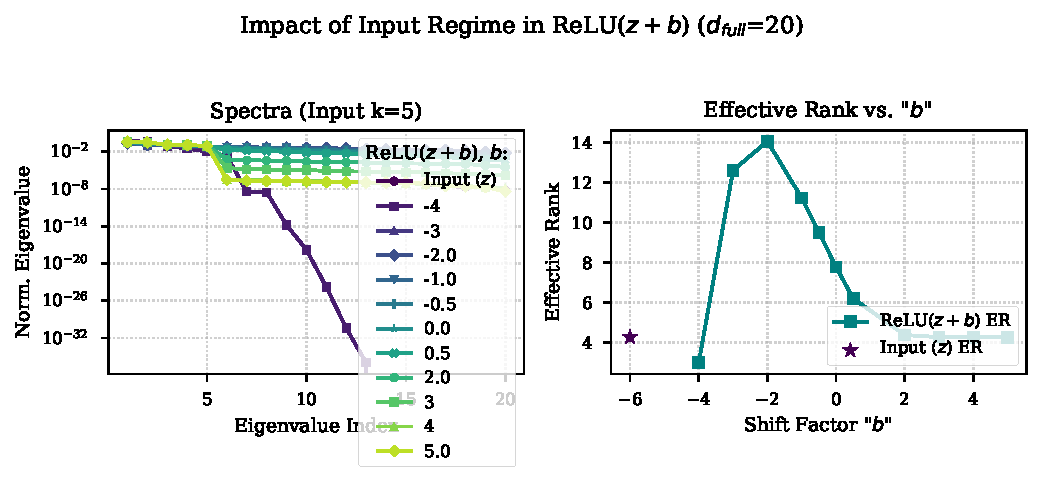
\includegraphics[width=0.7\linewidth]{figures/theory_relu_zb_rank.pdf}
    \caption{Effect of input shifting on post-activation effective rank for $h = \mathrm{ReLU}(z+b)$, with rank-deficient $z$. Large positive $b$ results in affine behavior, limiting rank recovery. Large negative $b$ causes rank collapse. An optimal $b$ (near zero for zero-mean $z$) maximizes non-linear effectiveness.}
    \label{fig:theory_relu_zb_rank_appendix}
\end{figure}

\begin{figure}[h!]
    \centering
    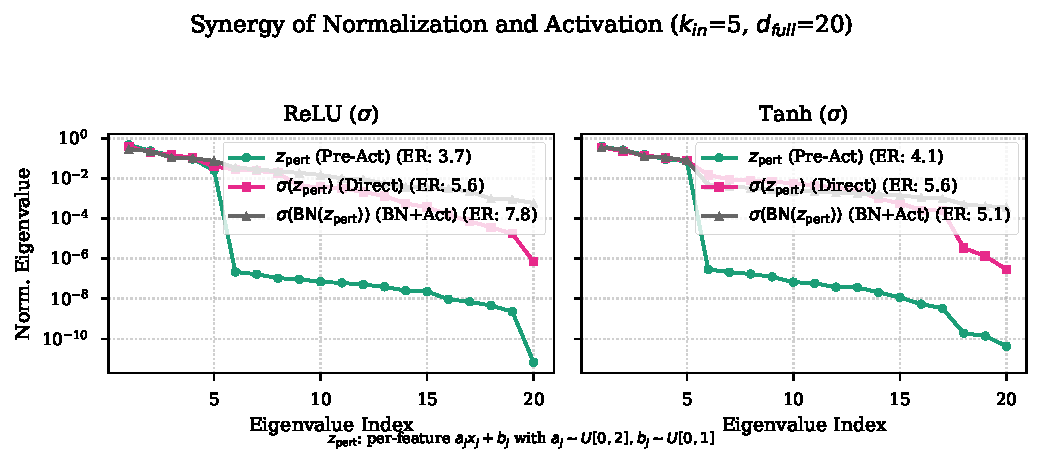
\includegraphics[width=0.7\linewidth]{figures/theory_joint_norm_activation_rank.pdf}
    \caption{Synergy of Batch Normalization (BN) with ReLU and Tanh for rank recovery from perturbed inputs. BN before activation consistently restores or enhances effective rank.}
    \label{fig:theory_joint_norm_activation_rank_appendix}
\end{figure}

\begin{figure}[h!]
    \centering
    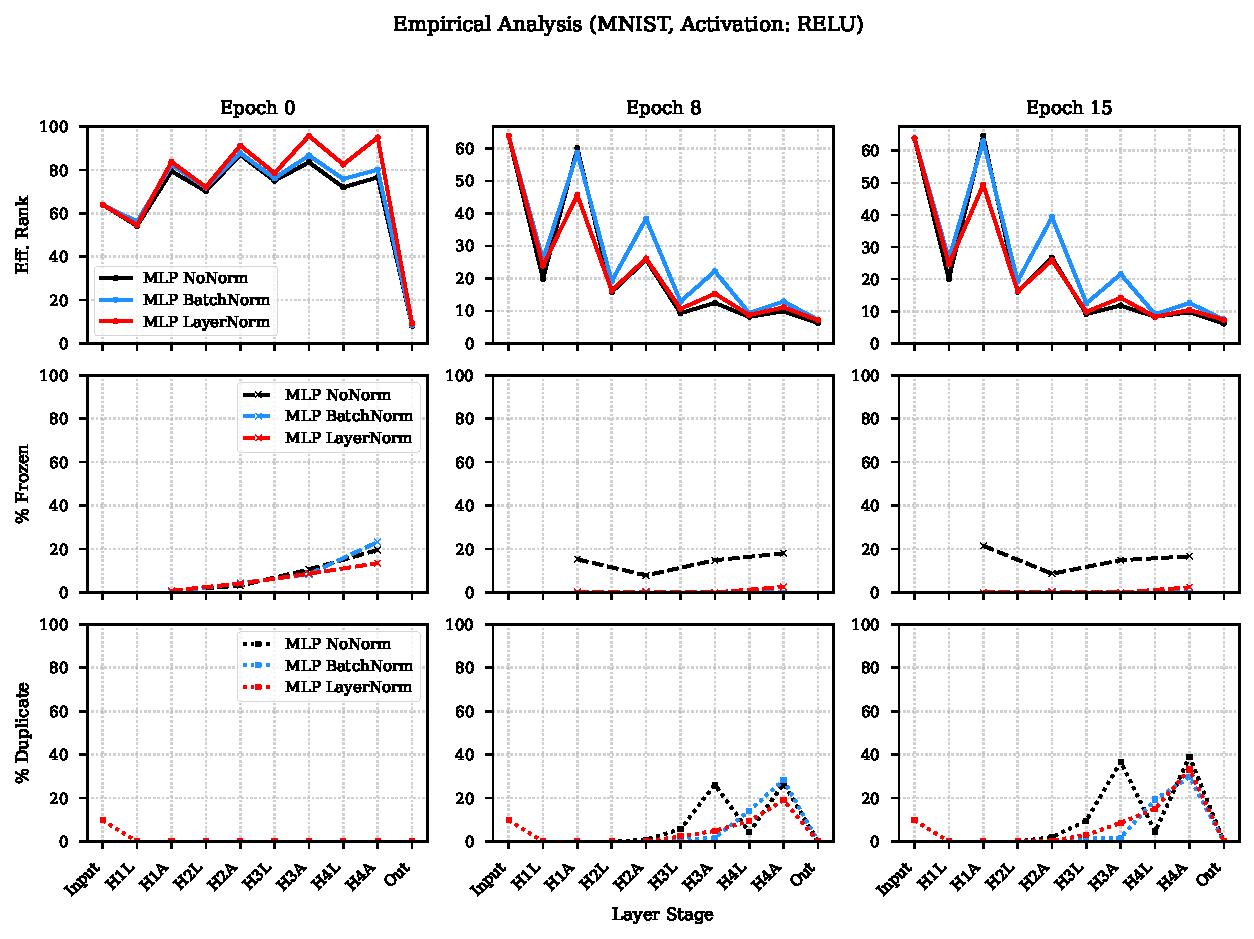
\includegraphics[width=\textwidth]{figures/empirical_all_metrics_ReLU_MNIST.pdf}
    \caption{Comprehensive empirical metrics for an MLP with ReLU activation trained on MNIST (Effective Rank, Frozen Units, Duplicate Units), comparing no normalization, BatchNorm, and LayerNorm at different epochs. Normalization generally improves these metrics.}
    \label{fig:empirical_all_metrics_appendix}
\end{figure}

\textbf{[Further details on datasets, architectures, hyperparameters, and specific metric calculations will be added here.]}

\end{document}